
\begin{figure}

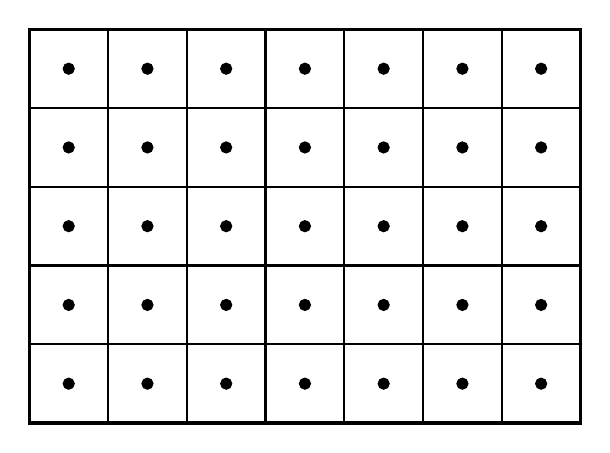
\begin{tikzpicture}

\def\lx{7}
\def\ly{5}

\draw[very thick] (0,0) rectangle (\lx,\ly);

\foreach \x in {1,...,6}
    \draw[thick] (\x,0) -- ++(0,\ly);

\foreach \y in {1,...,4}
    \draw[thick] (0,\y) -- ++(\lx,0);

\foreach \x in {1,...,7} {
    \foreach \y in {1,...,5} {
        \filldraw[] ({\x-0.5},{\y-0.5}) circle (2pt);
    }
}
% 
% \foreach \x in {1,...,7} {
%     \filldraw[] ({\x-0.5},0) circle (2pt);
%     \filldraw[] ({\x-0.5},\ly) circle (2pt);
% }
%
% \foreach \y in {1,...5} {
%     \filldraw[] (0,{\y-0.5}) circle (2pt);
%     \filldraw[] (\lx,{\y-0.5}) circle (2pt);
% }

% \filldraw[] (0,0) circle (2pt);
% \filldraw[] (0,\ly) circle (2pt);
% \filldraw[] (\lx,0) circle (2pt);
% \filldraw[] (\lx,\ly) circle (2pt);

\end{tikzpicture}

\end{figure}
